\section*{Website}
In its previous version, the accessibility of WOLF was limited to only ITTC members. Creating a website solution would allow anyone interested in running ML models easy access to WOLF. The goals in creating the website were to:
\begin{itemize}
	\item implement all of the features of the command line version
	\item keep the runs of all users separate
	\item make WOLF more user-friendly and intuitive
\end{itemize}

Much of the work for the website was planning out the goals and what a user should expect. Deciding on the file structure, a project timeline, and the visual layout were important in getting the work started. Once this began, Lei Wang worked on all of the user interface (UI) components and matching the layout for the goals that were put in place. My work on this involved making sure the initial setup of the SQL database for storing all runs of WOLF on the website was ready. The database also stored all model and dataset types and needed to be created in such a way that a new model or dataset could be added seamlessly and appear in website drop-down menus. For the runs, all users needed to have independent views. Each user should only be allowed to view their own runs and models. This was performed by having ``projects" that could be made public or private. The database is setup in a way that the owner of the project would also have the ability to add other collaborators to the project and allow them to make changes and perform their own runs.

Other work on the website included working on collecting model run data and putting it into tables for the 2017 IEEE International Conference on Big Data, at which other members of the team presented. A portion of the slides for the presentation \parencite{WOLFpresentation} were created using this data. Another portion of slides on related works, such as Auto-Weka and Michelangelo, were also created. All this information was also included in an unpublished report \parencite{WOLFpaper}.
\section*{Neural Network}
When this project began, deep learning was possible in WOLF with a Neural Network created using Caffe. Caffe is a framework developed by Berkeley AI Research for deep learning \parencite{Caffe}. It supports both CPU and GPU construction. In the past it had been a popular framework to use for creating neural networks, but in recent times it has been slowly falling out of use as data scientists are turning towards other libraries \parencite{NNrankings}. From the same site, it can be seen that the most popular frameworks are currently TensorFlow and PyTorch. Both of these are extremely popular in industry at this time, with TensorFlow showing no signs of stopping and PyTorch quickly rising.

PyTorch \parencite{PyTorch} is a framework built using Torch, which is a tensor library for GPUs. It is extremely helpful for creating reusable neural networks. The way that it runs is using ``reverse-mode auto-differentiation,'' which allows for changes to be made to the model with little overhead. PyTorch is meant to be easy to learn and has a strong community contributing to the open-source software. TensorFlow was created by Google as a way to perform computations on CPUs or GPUs \parencite{TensorFlow}. TensorFlow takes advantage of data flow graphs of computations and multi-dimensional arrays called tensors. Like PyTorch and Caffe, it can be used for end-to-end machine learning workflow creation. With the large market share that TensorFlow has, it is apparent that learning how to use it is valuable for working in industry. It would also be useful for a user to be able to train a neural network using TensorFlow.

With TensorFlow decided on, the best ways to integrate it into WOLF were explored. Keras appeared to be the best tool to use to implement a TensorFlow neural network. Keras \parencite{keras} is an API built to run on top of TensorFlow. Essentially it is a version of TensorFlow built for high level creation of neural networks. It is still the second most popular framework to build neural networks behind TensorFlow itself. Besides being extremely popular and manageable to understand, Keras also felt like Scikit-Learn \parencite{sklearn} in the way the function calls were set up, making it an easy transition in terms of syntax and fitting the calls into the WOLF model template style. To help write the code, a tutorial \parencite{KerasTutorial} was used.

Just like the Caffe version, the neural network models using TensorFlow and Keras allow for a selection of a variety of hyper-parameters. These hyper-parameters are:
\begin{itemize}
	\item the number of layers and nodes in each layer as a python list
	\item activation function
	\item input dropout
	\item hidden dropout
	\item learning rate
	\item number of epochs
	\item batch size
\end{itemize}


\section*{Saved Model and Predictions}
One major feature that WOLF was lacking was the ability to return a trained model to the user. As it stood in its previous form, there was only the ability to learn which hyper-parameters were the best for the dataset. When WOLF trains a model, it trains on each train/test data split pair. That means that a new model is created for each pair. When each model is trained, it is then saved to a file using pickle. For each hyper-parameter set, a folder is made with the same number of models as the dataset splits. The hyper-parameters with the best metrics allow for selection of the best of these models. The full path to the best pickled model is provided to the user in the results. If the user chooses to select a different model based on a different metric or a combination of multiple metrics, all models are still saved and one can match up the metric file with a model file to choose a different pickled file path than the results file provided.

Once a user chooses a model that they like, WOLF now allows a user to edit the configuration file to make predictions on a dataset. WOLF will read in the dataset, confirm it is in the correct form or try to format it if not, and then load the pickled model. Using this model, {\tt predict} can be called and the predictions can be written to a file that a user can download and use how they wish.

\section*{Feature Importance}
Once one has a trained model, it can be used to understand more about the dataset. A key area of model understanding is knowing the importance of each feature in the dataset. These values are the relative importance each feature of the dataset has on the prediction outcome of a model. That means these feature importance values are calculated from the model itself instead of from the dataset alone as feature extraction and feature selection do. If the model is good, these importances should line up with the overall importance of the feature in the dataset and real world. 

To calculate these importances, some models inherently have feature importance in the way the model works. These models, which have a built in attribute in {\tt sklearn} called {\tt feature\_importances\_}, are random forest, decision trees, and adaboost classifier. Other models required more work to calculate. For most others except for neural networks, the coefficients matrix could be used in the calculations. The coefficients matrix is an attribute, {\tt coef\_}, of many algorithms in the {\tt sklearn} library. The values in the matrix are positive if there is a correlation between the feature and the label being true and are negative if there is a correlation between the feature and the label being false. The further the value is from 0, the greater the correlation. To match the format of the models with the {\tt feature\_importances\_} attribute, {\tt coef\_} values need to be normalized between 0 and 1. The closer to 1 a value is, the more important the feature is. To normalize the values, the following equation is used, where \textit{Z} is the calculated importance value matrix and \textit{C} is the coefficient matrix: \[Z_i = \frac{|C_i| }{\sum_{j}|C_j|}\]

For the neural network using Keras, there is not a built in way to measure feature importance. Because of the complexity of neural networks, they are inherently not transparent or interpretable. There is much research being done in this area \parencite{Interpretable}, but in the meantime, a simpler, more brute force way of finding feature importance must be done. A common way to do this is to perform a ``leave one out" strategy \parencite{leaveoneout}. Because we do not want to train the model again for each feature, we instead can simulate taking out a feature by replacing all of the values with random values and making predictions on the training set. A package called ELI5 \parencite{eli5} was used for this. 

Once the feature importances are calculated, they are sorted and written to a file. Just like saving a model, this is done for each hyper-parameter combination and each train-test pair. All of the feature importance values are stored in a single file and the relative feature importances of the best configuration can be viewed in the main results file.

\section*{Datasets}
For showcasing the capability of WOLF at finding a model with optimal hyper-parameters, many datasets were downloaded from the UCI Machine Learning repository \parencite{UCIdata} that houses datasets for tasks of binary classification, multiclass classification, regression, and more. These datasets had to be downloaded and converted to {\tt arff} format while also confirming that the features and classes would work in WOLF or be able to pass through the pre-processing transaction to then work in WOLF. For binary and multiclass classification the datasets currently available are:
\begin{itemize}
	\item banknote
	\item breast cancer
	\item climate
	\item congress
	\item credit card
	\item dermatology (multiclass)
	\item diabetes
	\item fertility
	\item iris (multiclass)
	\item leaf (multiclass)
	\item pageblocks (multiclass)
	\item sonarmines
	\item spam
	\item transfusion
	\item vertebral
	\item voice rehab
	\item whitewine (multiclass)
	\item wholesale
\end{itemize}
The results of running WOLF can be seen in the results section.\newline

\section*{New Architecture}
After the implementation of these new features, the architecture of WOLF is changed from Figure \ref{fig:original WOLF workflow} to that in Figure \ref{fig:new WOLF workflow}. As can be seen in the graphic in green, saving models using pickle, feature importance, data prediction, and a neural network have been added. The website has also been added that incorporates every feature of WOLF. The prediction task is connected to the data by a dotted line as it is optional. It also is not connected to any of the other tasks, except for pickling a model. But this pickling must be done on a previous run of WOLF, otherwise the user will not know which model to tell WOLF to use.

\begin{figure}[H]
	\centering
	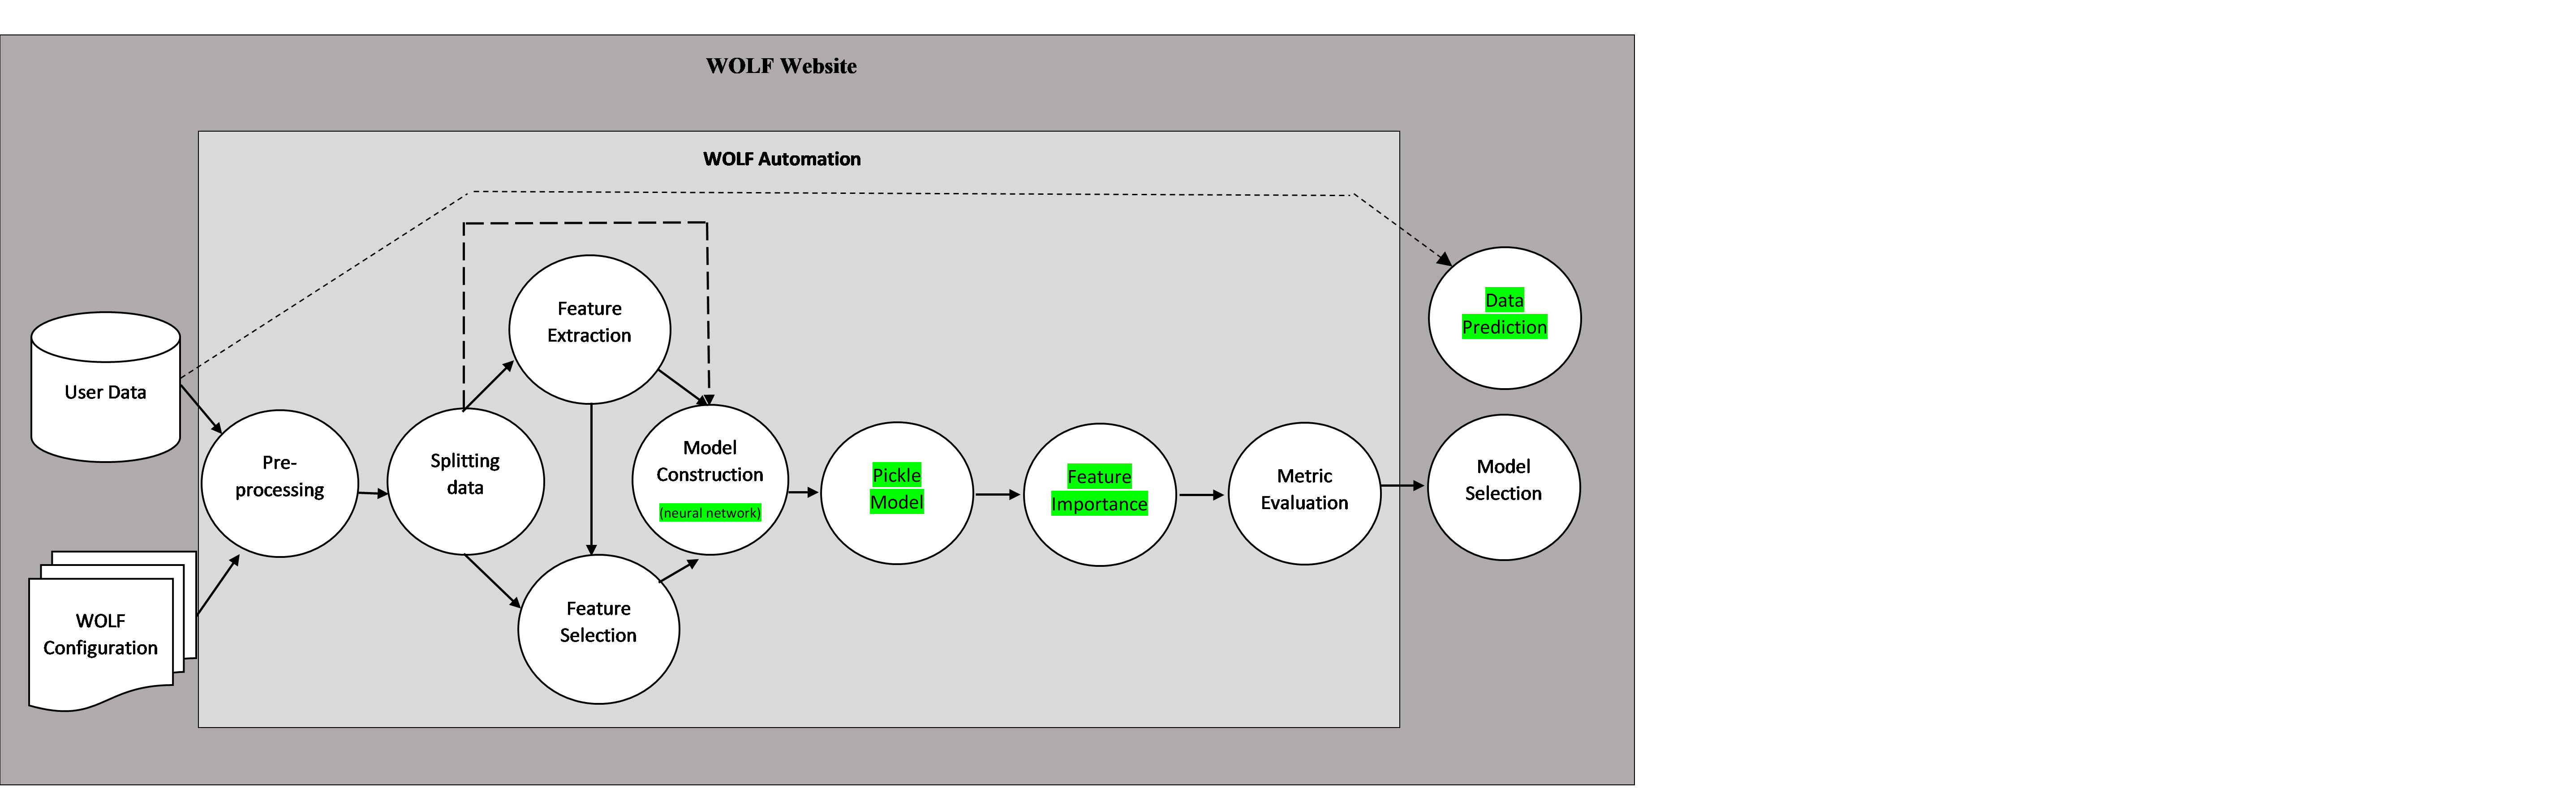
\includegraphics[scale=0.15]{new_arch}
	\caption{New WOLF architecture}
	\label{fig:new WOLF workflow}
\end{figure}

The MongoDB architecture has also changed slightly. Everything is the same as in Figure \ref{fig:original WOLF database} except for the Results database. The results database has gained two fields: {\tt model\_path} and {\tt feature\_importance\_path}. These are included so they can be passed to the metric collection and database results file and used appropriately for writing to the results excel file. The change can be seen in Figure \ref{fig:new WOLF database}.

\begin{figure}[H]
	\centering
	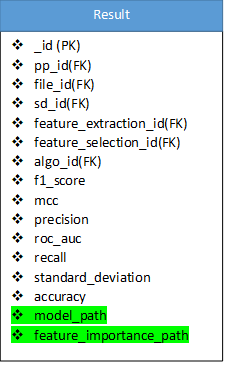
\includegraphics[scale=0.8]{new_db}
	\caption{New WOLF results database}
	\label{fig:new WOLF database}
\end{figure}